\begin{enumerate}
	\item L'utilisateur clique sur son nom dans la bar de navigation.
	\item L'utilisateur clique sur \textit{Profil} dans le menu déroulant.
	\item L'utilisateur clique sur le bouton edit au dessus de son profil. 
	\item Une fenêtre apparait. 
	\item L'utilisateur rentre les information qu'il souhaite changer. 
	\item L'utilisateur confirm en cliquant sur \textit{ok}
\end{enumerate}

\vspace{\baselineskip}
\begin{figure}[h]
	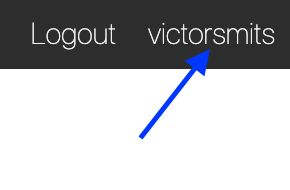
\includegraphics[width=0.4\textwidth,center]{Figures/us7-1}
	\caption{Bouton de navigation vers le profil}
\end{figure}

\begin{figure}[h]
	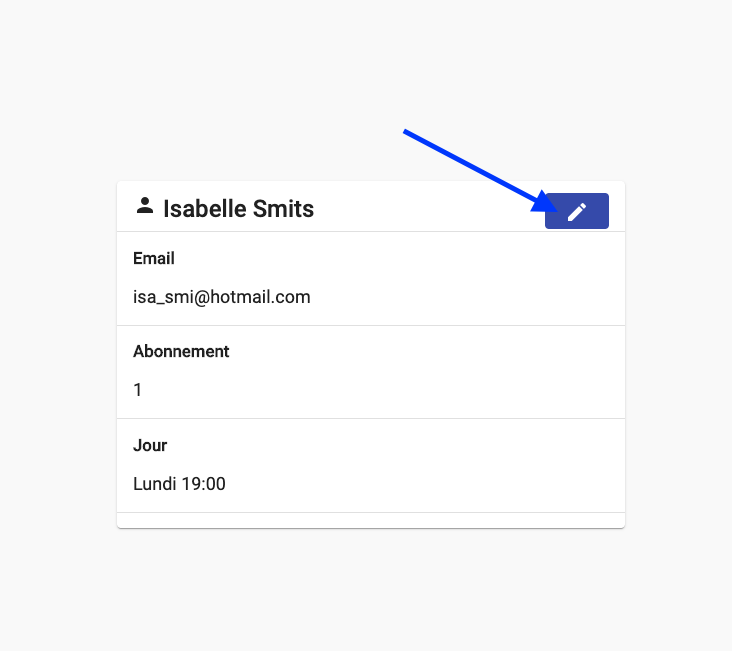
\includegraphics[width=0.4\textwidth,center]{Figures/us8-1}
	\caption{Bouton de modification du profil}
\end{figure}

\newpage
\begin{figure}[h]
	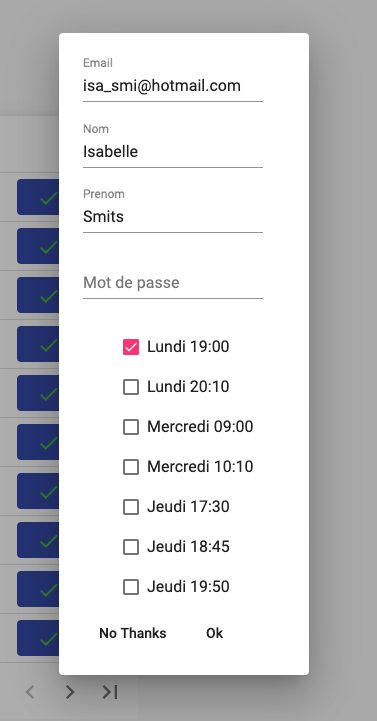
\includegraphics[width=0.4\textwidth,center]{Figures/us8-2}
	\caption{Fenêtre de modification des données du profil}
\end{figure}